\AppendixStyle{5.5em}
\section{\MakeUppercase{Appendices}}
    \setcounter{subsection}{0}
    \subsection{Project Schedule}
    \appendixnumbering{\Alph{subsection}}
    \label{app:project-schedule}

    \begin{figure}[H]
        \centering
        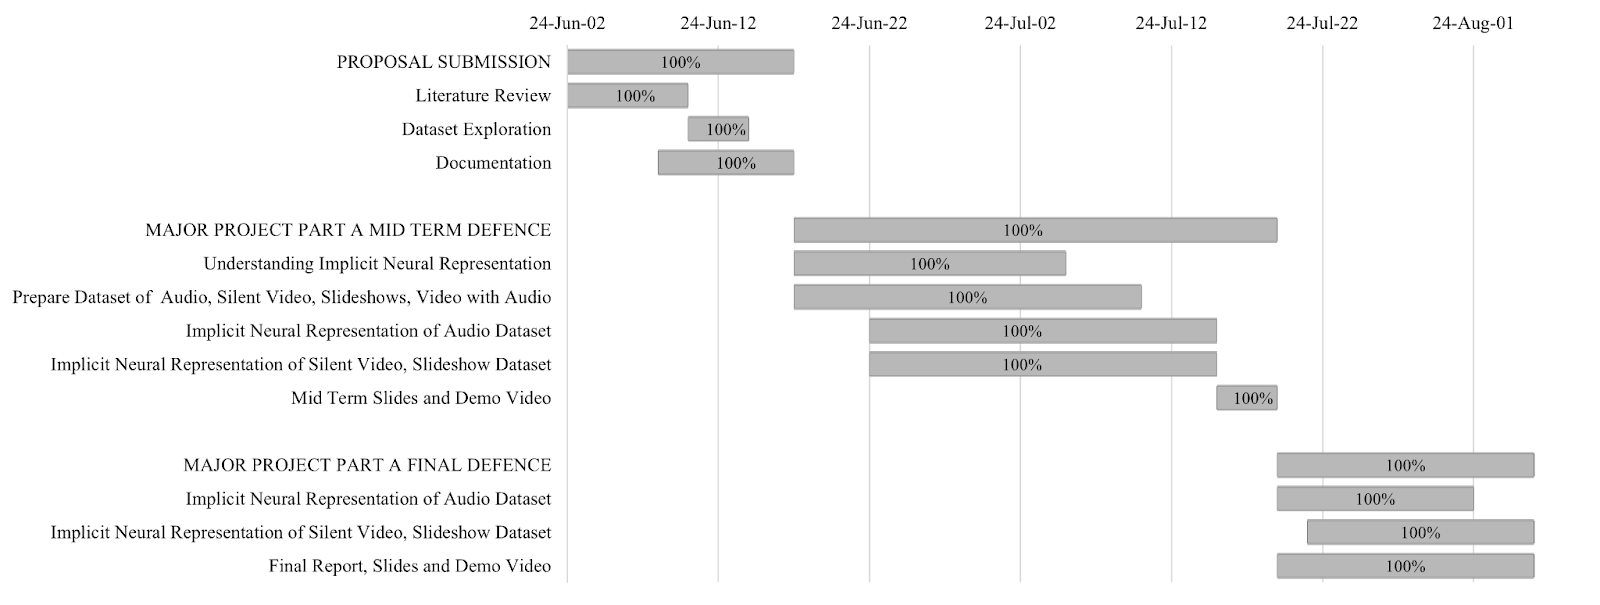
\includegraphics[angle=90, origin=c, height=0.5\textheight]{assets/Gantt-A.png}
        \caption{Gantt Chart for Major Project Part A}
        \label{fig:gantt-a}
    \end{figure}

    \begin{figure}[H]
        \centering
        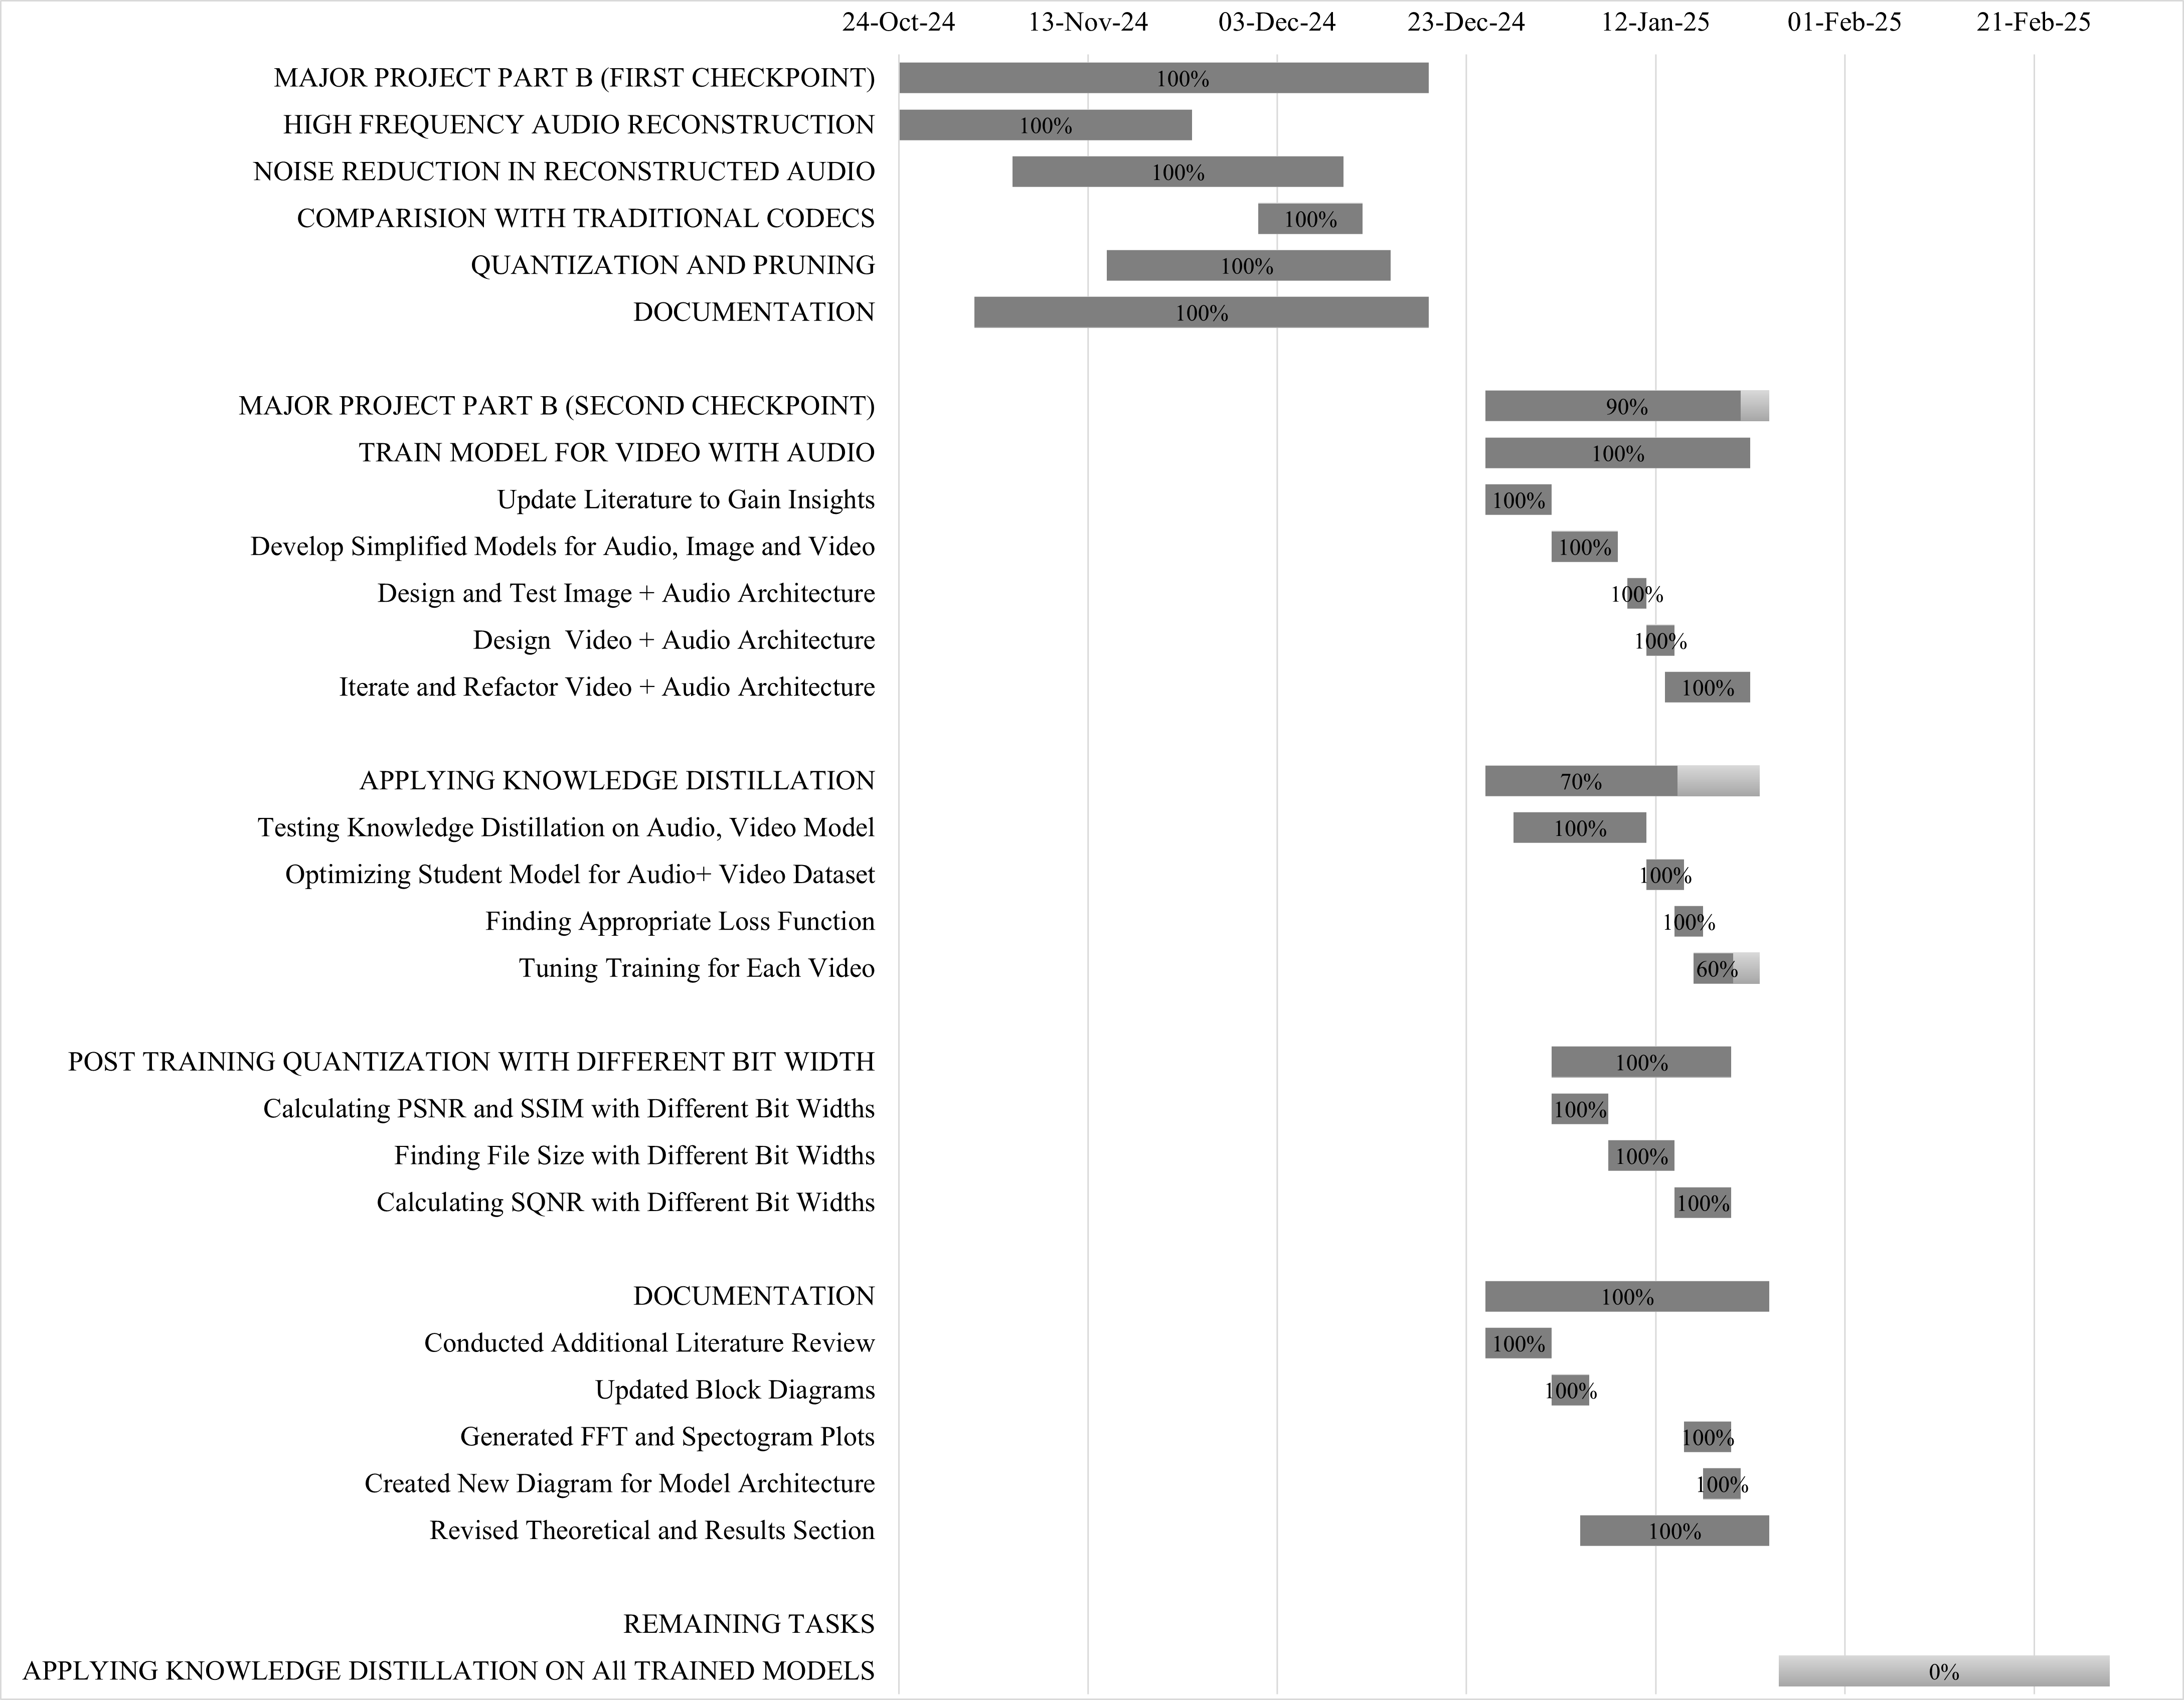
\includegraphics[angle=90, origin=c, height=0.7\textheight]{assets/Gantt-B.png}
        \caption{Gantt Chart for Major Project Part B}
        \label{fig:gantt-b}
    \end{figure}
    
\pagebreak


\setcounter{subsection}{1}
\subsection{Forward and Backward Propagation}
\appendixnumbering{\Alph{subsection}}
\label{app:forward-backward-eqn}

\begin{figure}[H]
    \centering
    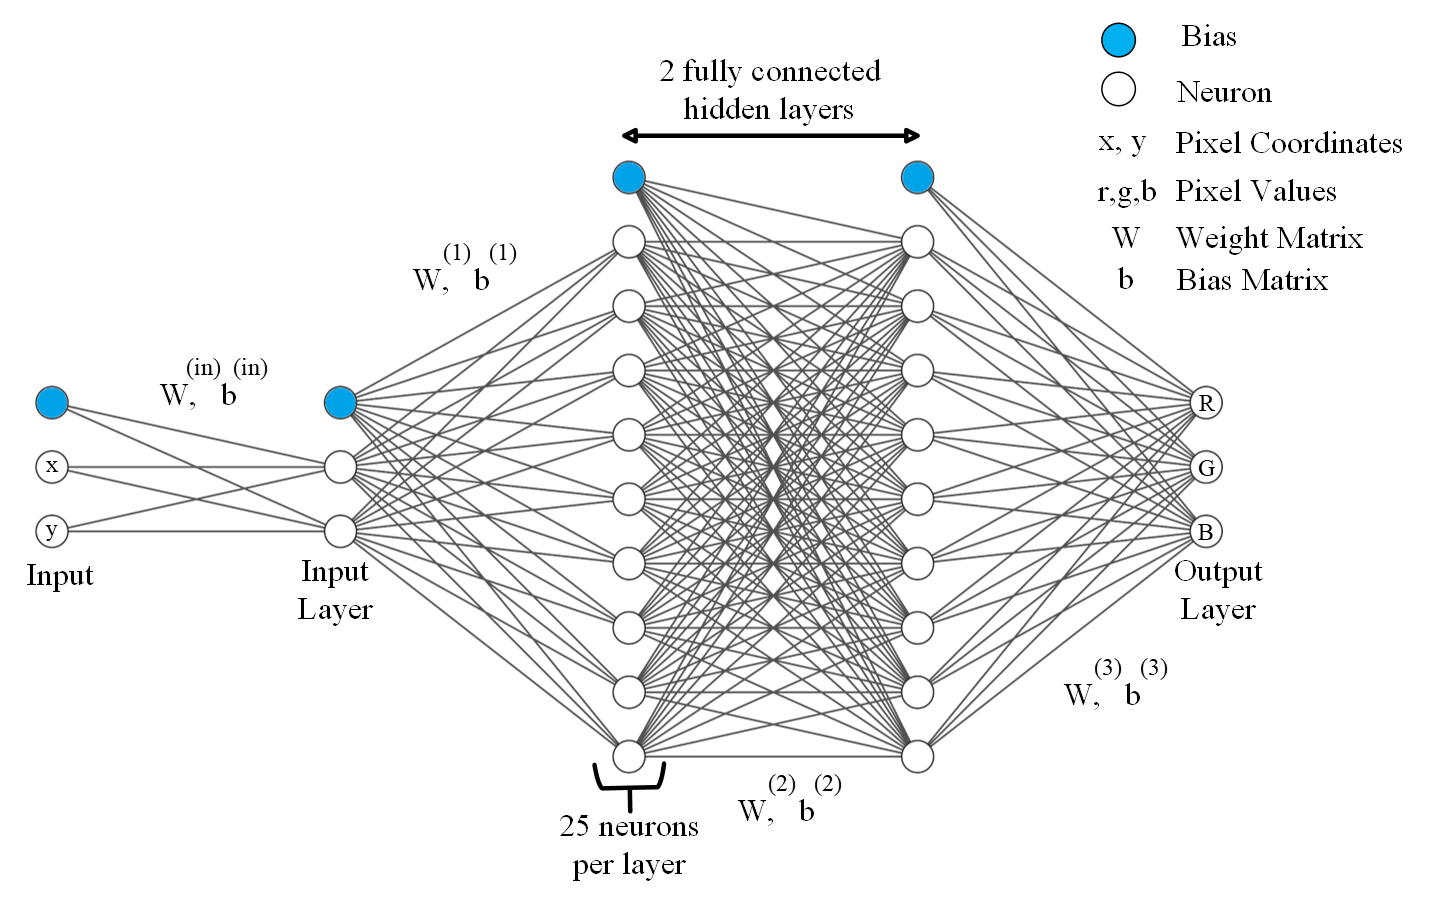
\includegraphics[width=\linewidth]{assets/32_32_neural.png}
    \caption{Neural Network Architecture for 32 by 32 image}
    \label{fig:32-32-neural}
\end{figure}

The below derivations have been done using \autoref{fig:32-32-neural} as reference.
\subsubsection{Forward Propagation}
\textbf{Step 1: Input Layer}
\begin{itemize}
  \item Input Vector $\mathbf{x}$: Dimension $2 \times 1$
  \item Weight Matrix $\mathbf{W}^{(in)}$: Dimension $2 \times 2$
  \item Bias Vector $\mathbf{b}^{(in)}$: Dimension $2 \times 1$
  \item Calculation:
  \begin{equation}
  \mathbf{z}^{(in)} = \mathbf{W}^{(in)} \mathbf{x} + \mathbf{b}^{(in)}
  \end{equation}
  \begin{equation}
  \mathbf{a}^{(in)} = \mathbf{z}^{(in)}
  \end{equation}
  Where $\mathbf{z}^{(in)}$ and $\mathbf{a}^{(in)}$ both have dimensions $2 \times 1$.
\end{itemize}


\textbf{Step 2: Hidden Layer 1}
\begin{itemize}
  \item Input Vector $\mathbf{x}$: Dimension $2 \times 1$
  \item Weight Matrix $\mathbf{W}^{(1)}$: Dimension $25 \times 2$
  \item Bias Vector $\mathbf{b}^{(1)}$: Dimension $25 \times 1$
  \item Calculation:
  \begin{equation}
  \mathbf{z}^{(1)} = \mathbf{W}^{(1)} \mathbf{x} + \mathbf{b}^{(1)}
  \end{equation}
  \begin{equation}
  \mathbf{a}^{(1)} = \sin(\mathbf{z}^{(1)})
  \end{equation}
  Where $\mathbf{z}^{(1)}$ and $\mathbf{a}^{(1)}$ both have dimensions $25 \times 1$.
\end{itemize}

\textbf{Step 3: Hidden Layer 2}
\begin{itemize}
  \item Weight Matrix $\mathbf{W}^{(2)}$: Dimension $25 \times 25$
  \item Bias Vector $\mathbf{b}^{(2)}$: Dimension $25 \times 1$
  \item Calculation:
  \begin{equation}
  \mathbf{z}^{(2)} = \mathbf{W}^{(2)} \mathbf{a}^{(1)} + \mathbf{b}^{(2)}
  \end{equation}
  \begin{equation}
  \mathbf{a}^{(2)} = \sin(\mathbf{z}^{(2)})
  \end{equation}
  Both $\mathbf{z}^{(2)}$ and $\mathbf{a}^{(2)}$ are $25 \times 1$.
\end{itemize}

\textbf{Step 4: Output Layer}
\begin{itemize}
  \item Weight Matrix $\mathbf{W}^{(3)}$: Dimension $3 \times 25$
  \item Bias Vector $\mathbf{b}^{(3)}$: Dimension $3 \times 1$
  \item Calculation:
  \begin{equation}
  \mathbf{z}^{(3)} = \mathbf{W}^{(3)} \mathbf{a}^{(2)} + \mathbf{b}^{(3)}
  \end{equation}
  \begin{equation}
  \mathbf{a}^{(3)} = \sin(\mathbf{z}^{(3)})
  \end{equation}
  Where $\mathbf{z}^{(3)}$ and $\mathbf{a}^{(3)}$ both have dimensions $3 \times 1$.
\end{itemize}


\subsubsection{Backpropagation}

\textbf{Step 1: Output Layer}
\begin{enumerate}[label=\textbf{\roman*.}]
  \item \textbf{Gradient of Loss with respect to output activations} $(\mathbf{a}^{(3)})$:
  
  Given the Mean Squared Error (MSE) loss function:
  \begin{equation}
  \text{Loss} = \frac{1}{2} \sum_{i=1}^{3} (y_i - a^{(3)}_i)^2
  \end{equation}
  Differentiate Loss w.r.t. $\mathbf{a}^{(3)}$:
  \begin{equation}
  \frac{\partial \text{Loss}}{\partial a^{(3)}_i} = a^{(3)}_i - y_i
  \end{equation}
  This will result in a vector $\mathbf{a}^{(3)} - \mathbf{y}$.

  \item \textbf{Gradient with respect to} $\mathbf{z}^{(3)}$ (using chain rule and recognizing $\mathbf{a}^{(3)} = \sin(\mathbf{z}^{(3)})$):
  \[
  \frac{\partial \text{Loss}}{\partial \mathbf{z}^{(3)}} = \frac{\partial \text{Loss}}{\partial \mathbf{a}^{(3)}} \cdot \frac{\partial \mathbf{a}^{(3)}}{\partial \mathbf{z}^{(3)}}
  \]
  Since $\frac{\partial a^{(3)}_i}{\partial z^{(3)}_i} = \cos(z^{(3)}_i)$, the gradient becomes:
  \begin{equation}
  \frac{\partial \text{Loss}}{\partial \mathbf{z}^{(3)}} = (\mathbf{a}^{(3)} - \mathbf{y}) \cdot \cos(\mathbf{z}^{(3)})
  \end{equation}

  \item \textbf{Gradient with respect to weights} $\mathbf{W}^{(3)}$ \textbf{and biases} $\mathbf{b}^{(3)}$:
  
  \[
  \frac{\partial \text{Loss}}{\partial \mathbf{W}^{(3)}} = \frac{\partial \text{Loss}}{\partial \mathbf{z}^{(3)}} \cdot \frac{\partial \mathbf{z}^{(3)}}{\partial \mathbf{W}^{(3)}}
  \]
  
  \[
  \frac{\partial \text{Loss}}{\partial \mathbf{W}^{(3)}} = \frac{\partial \text{Loss}}{\partial \mathbf{z}^{(3)}} \mathbf{a}^{(2)T}
  \]
  
  \begin{equation}
  \frac{\partial \text{Loss}}{\partial \mathbf{W}^{(3)}} = \left((\mathbf{a}^{(3)} - \mathbf{y}) \cdot \cos(\mathbf{z}^{(3)})\right) \mathbf{a}^{(2)T}
  \end{equation}


  \[
  \frac{\partial \text{Loss}}{\partial \mathbf{b}^{(3)}} = \frac{\partial \text{Loss}}{\partial \mathbf{z}^{(3)}} \cdot \frac{\partial \mathbf{z}^{(3)}}{\partial \mathbf{b}^{(3)}}
  \]

  \[
  \frac{\partial \text{Loss}}{\partial \mathbf{b}^{(3)}} = \frac{\partial \text{Loss}}{\partial \mathbf{z}^{(3)}}
  \]

  \begin{equation}
  \frac{\partial \text{Loss}}{\partial \mathbf{b}^{(3)}} = (\mathbf{a}^{(3)} - \mathbf{y}) \cdot \cos(\mathbf{z}^{(3)})
  \end{equation}
  
\end{enumerate}

\textbf{Step 2: Hidden Layer 2}
\begin{enumerate}[label=\textbf{\roman*.}]
  \item \textbf{Gradient with respect to activations} $\mathbf{a}^{(2)}$:
    \[
  \frac{\partial \text{Loss}}{\partial \mathbf{a}^{(2)}} = \frac{\partial \text{Loss}}{\partial \mathbf{z}^{(3)}} \cdot \frac{\partial \mathbf{z}^{(3)}}{\partial \mathbf{a}^{(2)}}
  \]
  \[
  \frac{\partial \text{Loss}}{\partial \mathbf{a}^{(2)}} = \mathbf{W}^{(3)T} \frac{\partial \text{Loss}}{\partial \mathbf{z}^{(3)}}
  \]
  \begin{equation}
  \frac{\partial \text{Loss}}{\partial \mathbf{a}^{(2)}} = \mathbf{W}^{(3)T} \left((\mathbf{a}^{(3)} - \mathbf{y}) \cdot \cos(\mathbf{z}^{(3)})\right)
  \end{equation}
  \item \textbf{Gradient with respect to} $\mathbf{z}^{(2)}$:
    \[
  \frac{\partial \text{Loss}}{\partial \mathbf{z}^{(2)}} = \frac{\partial \text{Loss}}{\partial \mathbf{a}^{(2)}} \cdot \frac{\partial \mathbf{a}^{(2)}}{\partial \mathbf{z}^{(2)}}
  \]
  \[
  \frac{\partial \text{Loss}}{\partial \mathbf{z}^{(2)}} = \frac{\partial \text{Loss}}{\partial \mathbf{a}^{(2)}} \cdot \cos(\mathbf{z}^{(2)})
  \]
  \begin{equation}
  \frac{\partial \text{Loss}}{\partial \mathbf{z}^{(2)}} = \left(\mathbf{W}^{(3)T} \left((\mathbf{a}^{(3)} - \mathbf{y}) \cdot \cos(\mathbf{z}^{(3)})\right)\right) \cdot \cos(\mathbf{z}^{(2)})
  \end{equation}

  \item \textbf{Gradient with respect to weights} $\mathbf{W}^{(2)}$ \textbf{and biases} $\mathbf{b}^{(2)}$:
  \[
  \frac{\partial \text{Loss}}{\partial \mathbf{W}^{(2)}} = \frac{\partial \text{Loss}}{\partial \mathbf{z}^{(2)}} \cdot \frac{\partial \mathbf{z}^{(2)}}{\partial \mathbf{W}^{(2)}}
  \]
  \[
  \frac{\partial \text{Loss}}{\partial \mathbf{W}^{(2)}} = \frac{\partial \text{Loss}}{\partial \mathbf{z}^{(2)}} \mathbf{a}^{(1)T}
  \]

  \begin{equation}
  \frac{\partial \text{Loss}}{\partial \mathbf{W}^{(2)}} = \left(\left(\mathbf{W}^{(3)T} \left((\mathbf{a}^{(3)} - \mathbf{y}) \cdot \cos(\mathbf{z}^{(3)})\right)\right) \cdot \cos(\mathbf{z}^{(2)})\right) \mathbf{a}^{(1)T}
  \end{equation}
 

   \[
  \frac{\partial \text{Loss}}{\partial \mathbf{b}^{(2)}} = \frac{\partial \text{Loss}}{\partial \mathbf{z}^{(2)}} \cdot \frac{\partial \mathbf{z}^{(2)}}{\partial \mathbf{b}^{(2)}}
  \]
  \[
  \frac{\partial \text{Loss}}{\partial \mathbf{b}^{(2)}} = \frac{\partial \text{Loss}}{\partial \mathbf{z}^{(2)}}
  \]

  \begin{equation}
  \frac{\partial \text{Loss}}{\partial \mathbf{b}^{(2)}} = \left(\mathbf{W}^{(3)T} \left((\mathbf{a}^{(3)} - \mathbf{y}) \cdot \cos(\mathbf{z}^{(3)})\right)\right) \cdot \cos(\mathbf{z}^{(2)})
  \end{equation}
\end{enumerate}

\textbf{Step 3: Hidden Layer 1}
\begin{enumerate}[label=\textbf{\roman*.}]
  \item \textbf{Gradient with respect to activations} $\mathbf{a}^{(1)}$:
      \[
  \frac{\partial \text{Loss}}{\partial \mathbf{a}^{(1)}} = \frac{\partial \text{Loss}}{\partial \mathbf{z}^{(2)}} \cdot \frac{\partial \mathbf{z}^{(2)}}{\partial \mathbf{a}^{(1)}}
  \]
  
  \[
  \frac{\partial \text{Loss}}{\partial \mathbf{a}^{(1)}} = \mathbf{W}^{(2)T} \frac{\partial \text{Loss}}{\partial \mathbf{z}^{(2)}}
  \]
  \begin{equation}
  \frac{\partial \text{Loss}}{\partial \mathbf{a}^{(1)}} = \mathbf{W}^{(2)T} \left(\left(\mathbf{W}^{(3)T} \left((\mathbf{a}^{(3)} - \mathbf{y}) \cdot \cos(\mathbf{z}^{(3)})\right)\right) \cdot \cos(\mathbf{z}^{(2)})\right)
  \end{equation}

  \item \textbf{Gradient with respect to} $\mathbf{z}^{(1)}$:
    \[
  \frac{\partial \text{Loss}}{\partial \mathbf{z}^{(1)}} = \frac{\partial \text{Loss}}{\partial \mathbf{a}^{(1)}} \cdot \frac{\partial \mathbf{a}^{(1)}}{\partial \mathbf{z}^{(1)}}
  \]

  \[
  \frac{\partial \text{Loss}}{\partial \mathbf{z}^{(1)}} = \frac{\partial \text{Loss}}{\partial \mathbf{a}^{(1)}} \cdot \cos(\mathbf{z}^{(1)})
  \]
  \begin{equation}
  \frac{\partial \text{Loss}}{\partial \mathbf{z}^{(1)}} = \left(\mathbf{W}^{(2)T} \left(\left(\mathbf{W}^{(3)T} \left((\mathbf{a}^{(3)} - \mathbf{y}) \cdot \cos(\mathbf{z}^{(3)})\right)\right) \cdot \cos(\mathbf{z}^{(2)})\right)\right) \cdot \cos(\mathbf{z}^{(1)})
  \end{equation}

  \item \textbf{Gradient with respect to weights} $\mathbf{W}^{(1)}$ \textbf{and biases} $\mathbf{b}^{(1)}$:
       \[
  \frac{\partial \text{Loss}}{\partial \mathbf{W}^{(1)}} = \frac{\partial \text{Loss}}{\partial \mathbf{z}^{(1)}} \cdot \frac{\partial \mathbf{z}^{(1)}}{\partial \mathbf{W}^{(1)}}
  \]
  \[
  \frac{\partial \text{Loss}}{\partial \mathbf{W}^{(1)}} = \frac{\partial \text{Loss}}{\partial \mathbf{z}^{(1)}} \mathbf{x}^T
  \]
  \begin{equation}
  \frac{\partial \text{Loss}}{\partial \mathbf{W}^{(1)}} = \left(\left(\mathbf{W}^{(2)T} \left(\left(\mathbf{W}^{(3)T} \left((\mathbf{a}^{(3)} - \mathbf{y}) \cdot \cos(\mathbf{z}^{(3)})\right)\right) \cdot \cos(\mathbf{z}^{(2)})\right)\right) \cdot \cos(\mathbf{z}^{(1)})\right) \mathbf{x}^T
  \end{equation}

  
         \[
  \frac{\partial \text{Loss}}{\partial \mathbf{b}^{(1)}} = \frac{\partial \text{Loss}}{\partial \mathbf{z}^{(1)}} \cdot \frac{\partial \mathbf{z}^{(1)}}{\partial \mathbf{b}^{(1)}}
  \]
  \[
  \frac{\partial \text{Loss}}{\partial \mathbf{b}^{(1)}} = \frac{\partial \text{Loss}}{\partial \mathbf{z}^{(1)}}
  \]
  \begin{equation}
  \frac{\partial \text{Loss}}{\partial \mathbf{b}^{(1)}} = \left(\mathbf{W}^{(2)T} \left(\left(\mathbf{W}^{(3)T} \left((\mathbf{a}^{(3)} - \mathbf{y}) \cdot \cos(\mathbf{z}^{(3)})\right)\right) \cdot \cos(\mathbf{z}^{(2)})\right)\right) \cdot \cos(\mathbf{z}^{(1)})
  \end{equation}
\end{enumerate}

\textbf{Step 4: Input Layer}
\begin{enumerate}[label=\textbf{\roman*.}]
  \item \textbf{Gradient with respect to activations} $\mathbf{a}^{(in)}$:
      \[
  \frac{\partial \text{Loss}}{\partial \mathbf{a}^{(in)}} = \frac{\partial \text{Loss}}{\partial \mathbf{z}^{(1)}} \cdot \frac{\partial \mathbf{z}^{(1)}}{\partial \mathbf{a}^{(in)}}
  \]
  
  \[
  \frac{\partial \text{Loss}}{\partial \mathbf{a}^{(in)}} = \mathbf{W}^{(1)T} \frac{\partial \text{Loss}}{\partial \mathbf{z}^{(1)}}
  \]
  \begin{equation}
  \frac{\partial \text{Loss}}{\partial \mathbf{a}^{(in)}} =\mathbf{W}^{(1)T}\left(\left(\mathbf{W}^{(2)T} \left(\left(\mathbf{W}^{(3)T} \left((\mathbf{a}^{(3)} - \mathbf{y}) \cdot \cos(\mathbf{z}^{(3)})\right)\right) \cdot \cos(\mathbf{z}^{(2)})\right)\right) \cdot \cos(\mathbf{z}^{(1)})\right) 
  \end{equation}

  \item \textbf{Gradient with respect to} $\mathbf{z}^{(in)}$:
    \[
  \frac{\partial \text{Loss}}{\partial \mathbf{z}^{(in)}} = \frac{\partial \text{Loss}}{\partial \mathbf{a}^{(in)}} \cdot \frac{\partial \mathbf{a}^{(in)}}{\partial \mathbf{z}^{(in)}}
  \]

  \[
  \frac{\partial \text{Loss}}{\partial \mathbf{z}^{(in)}} = \frac{\partial \text{Loss}}{\partial \mathbf{a}^{(in)}} \cdot \cos(\mathbf{z}^{(in)})
  \]
  \begin{equation}
  \frac{\partial \text{Loss}}{\partial \mathbf{z}^{(in)}} = \mathbf{W}^{(1)T}\left(\left(\mathbf{W}^{(2)T} \left(\left(\mathbf{W}^{(3)T} \left((\mathbf{a}^{(3)} - \mathbf{y}) \cdot \cos(\mathbf{z}^{(3)})\right)\right) \cdot \cos(\mathbf{z}^{(2)})\right)\right) \cdot \cos(\mathbf{z}^{(1)})\right)  \cdot \cos(\mathbf{z}^{(in)})
  \end{equation}

  \item \textbf{Gradient with respect to weights} $\mathbf{W}^{(in)}$ \textbf{and biases} $\mathbf{b}^{(in)}$:
       \[
  \frac{\partial \text{Loss}}{\partial \mathbf{W}^{(in)}} = \frac{\partial \text{Loss}}{\partial \mathbf{z}^{(in)}} \cdot \frac{\partial \mathbf{z}^{(in)}}{\partial \mathbf{W}^{(in)}}
  \]
  \begin{equation}
  \frac{\partial \text{Loss}}{\partial \mathbf{W}^{(in)}} = \frac{\partial \text{Loss}}{\partial \mathbf{z}^{(in)}} \mathbf{x}^T
  \end{equation}
  %   \[
  % \frac{\partial \text{Loss}}{\partial \mathbf{W}^{(in)}} = \mathbf{W}^{(1)T}\left(\left(\mathbf{W}^{(2)T} \left(\left(\mathbf{W}^{(3)T} \left((\mathbf{a}^{(3)} - \mathbf{y}) \cdot \cos(\mathbf{z}^{(3)})\right)\right) \cdot \cos(\mathbf{z}^{(2)})\right)\right) \cdot \cos(\mathbf{z}^{(1)})\right)  \cdot \cos(\mathbf{z}^{(in)}) \mathbf{x}^T
  % \]

         \[
  \frac{\partial \text{Loss}}{\partial \mathbf{b}^{(in)}} = \frac{\partial \text{Loss}}{\partial \mathbf{z}^{(in)}} \cdot \frac{\partial \mathbf{z}^{(in)}}{\partial \mathbf{b}^{(in)}}
  \]
  \begin{equation}
  \frac{\partial \text{Loss}}{\partial \mathbf{b}^{(in)}} = \frac{\partial \text{Loss}}{\partial \mathbf{z}^{(in)}}
  \end{equation}
% \[
%   \frac{\partial \text{Loss}}{\partial \mathbf{b}^{(in)}} = \mathbf{W}^{(1)T}\left(\left(\mathbf{W}^{(2)T} \left(\left(\mathbf{W}^{(3)T} \left((\mathbf{a}^{(3)} - \mathbf{y}) \cdot \cos(\mathbf{z}^{(3)})\right)\right) \cdot \cos(\mathbf{z}^{(2)})\right)\right) \cdot \cos(\mathbf{z}^{(1)})\right)  \cdot \cos(\mathbf{z}^{(in)})
%   \]
\end{enumerate}

\pagebreak


\setcounter{subsection}{2}
\subsection{Arcsine Distribution on [-1, 1]}
\label{app:arcsine-distribution}
\appendixnumbering{\Alph{subsection}}

\textbf{Probability Density Function (PDF)}\\
The PDF of the arcsine distribution on the interval \((-1, 1)\) is given by:
\begin{equation}
    f(x) = \frac{1}{\pi \sqrt{1-x^2}}
\end{equation}

\textbf{Cumulative Distribution Function (CDF)}\\
The cumulative distribution function (CDF), \( F(x) \), is defined as the integral of the probability density function (PDF) from the lower bound of the interval to \( x \):
\begin{equation}
    F(x) = \int_{-1}^{x} f(t) \, dt
\end{equation}

Given the PDF for the arcsine distribution:
\[
f(x) = \frac{1}{\pi \sqrt{1-x^2}}
\]

we need to integrate this PDF from -1 to \( x \):
\[
F(x) = \int_{-1}^{x} \frac{1}{\pi \sqrt{1-t^2}} \, dt
\]

To solve this integral, we use the substitution \( t = \sin \theta \).\\
Thus, \( dt = \cos \theta \, d\theta \) and \( \sqrt{1-t^2} = \sqrt{1-\sin^2 \theta} = \cos \theta \).\\
When \( t = -1 \), \( \theta = -\frac{\pi}{2} \).\\
When \( t = x \), \( \theta = \arcsin x \).\\
Therefore, the integral becomes:
\[
F(x) = \int_{-\frac{\pi}{2}}^{\arcsin x} \frac{1}{\pi \cos \theta} \cos \theta \, d\theta = \int_{-\frac{\pi}{2}}^{\arcsin x} \frac{1}{\pi} \, d\theta
\]

\[
F(x) = \frac{1}{\pi} \int_{-\frac{\pi}{2}}^{\arcsin x} d\theta = \frac{1}{\pi} \left[ \theta \right]_{-\frac{\pi}{2}}^{\arcsin x}
\]

\[
F(x) = \frac{1}{\pi} \left( \arcsin x - \left( -\frac{\pi}{2} \right) \right)
\]

\[
F(x) = \frac{1}{\pi} \arcsin x + \frac{1}{\pi} \cdot \frac{\pi}{2}
\]

\[
F(x) = \frac{1}{\pi} \arcsin x + \frac{1}{2}
\]

Thus, the CDF of the arcsine distribution on \([-1, 1]\) is:
\begin{equation}
    F(x) = \frac{1}{\pi} \arcsin(x) + \frac{1}{2}
\end{equation}

\textbf{Mean}\\
The mean \(\mu\) of the distribution is given by:
\begin{equation}
    \mu = \int_{-1}^{1} x f(x) \, dx = \int_{-1}^{1} x \cdot \frac{1}{\pi \sqrt{1-x^2}} \, dx
\end{equation}
This integral evaluates to zero because \( x \cdot f(x) \) is an odd function integrated over a symmetric interval around zero:
\begin{equation}
    \mu = 0
\end{equation}

\textbf{Variance}\\
The variance \(\sigma^2\) is calculated as:
\begin{equation}
    \sigma^2 = \mathbf{E}[X^2] - (\mathbf{E}[X])^2
\end{equation}
Since \(\mathbf{E}[X] = 0\), we have:
\[
\mathbf{E}[X^2] = \int_{-1}^{1} x^2 f(x) \, dx = \int_{-1}^{1} x^2 \cdot \frac{1}{\pi \sqrt{1-x^2}} \, dx
\]
By symmetry and properties of the arcsine distribution, this integral evaluates to:
\[
\mathbf{E}[X^2] = \frac{1}{2}
\]
Thus, the variance is:
\begin{equation}
    \sigma^2 = \frac{1}{2} - 0^2 = \frac{1}{2}
\end{equation}

\pagebreak

\setcounter{subsection}{3}
\subsection{IEEE 754 Floating Point Representation}
\label{app:ieee-754-fp32}
\appendixnumbering{\Alph{subsection}}

\begin{figure}[H]
    \centering
    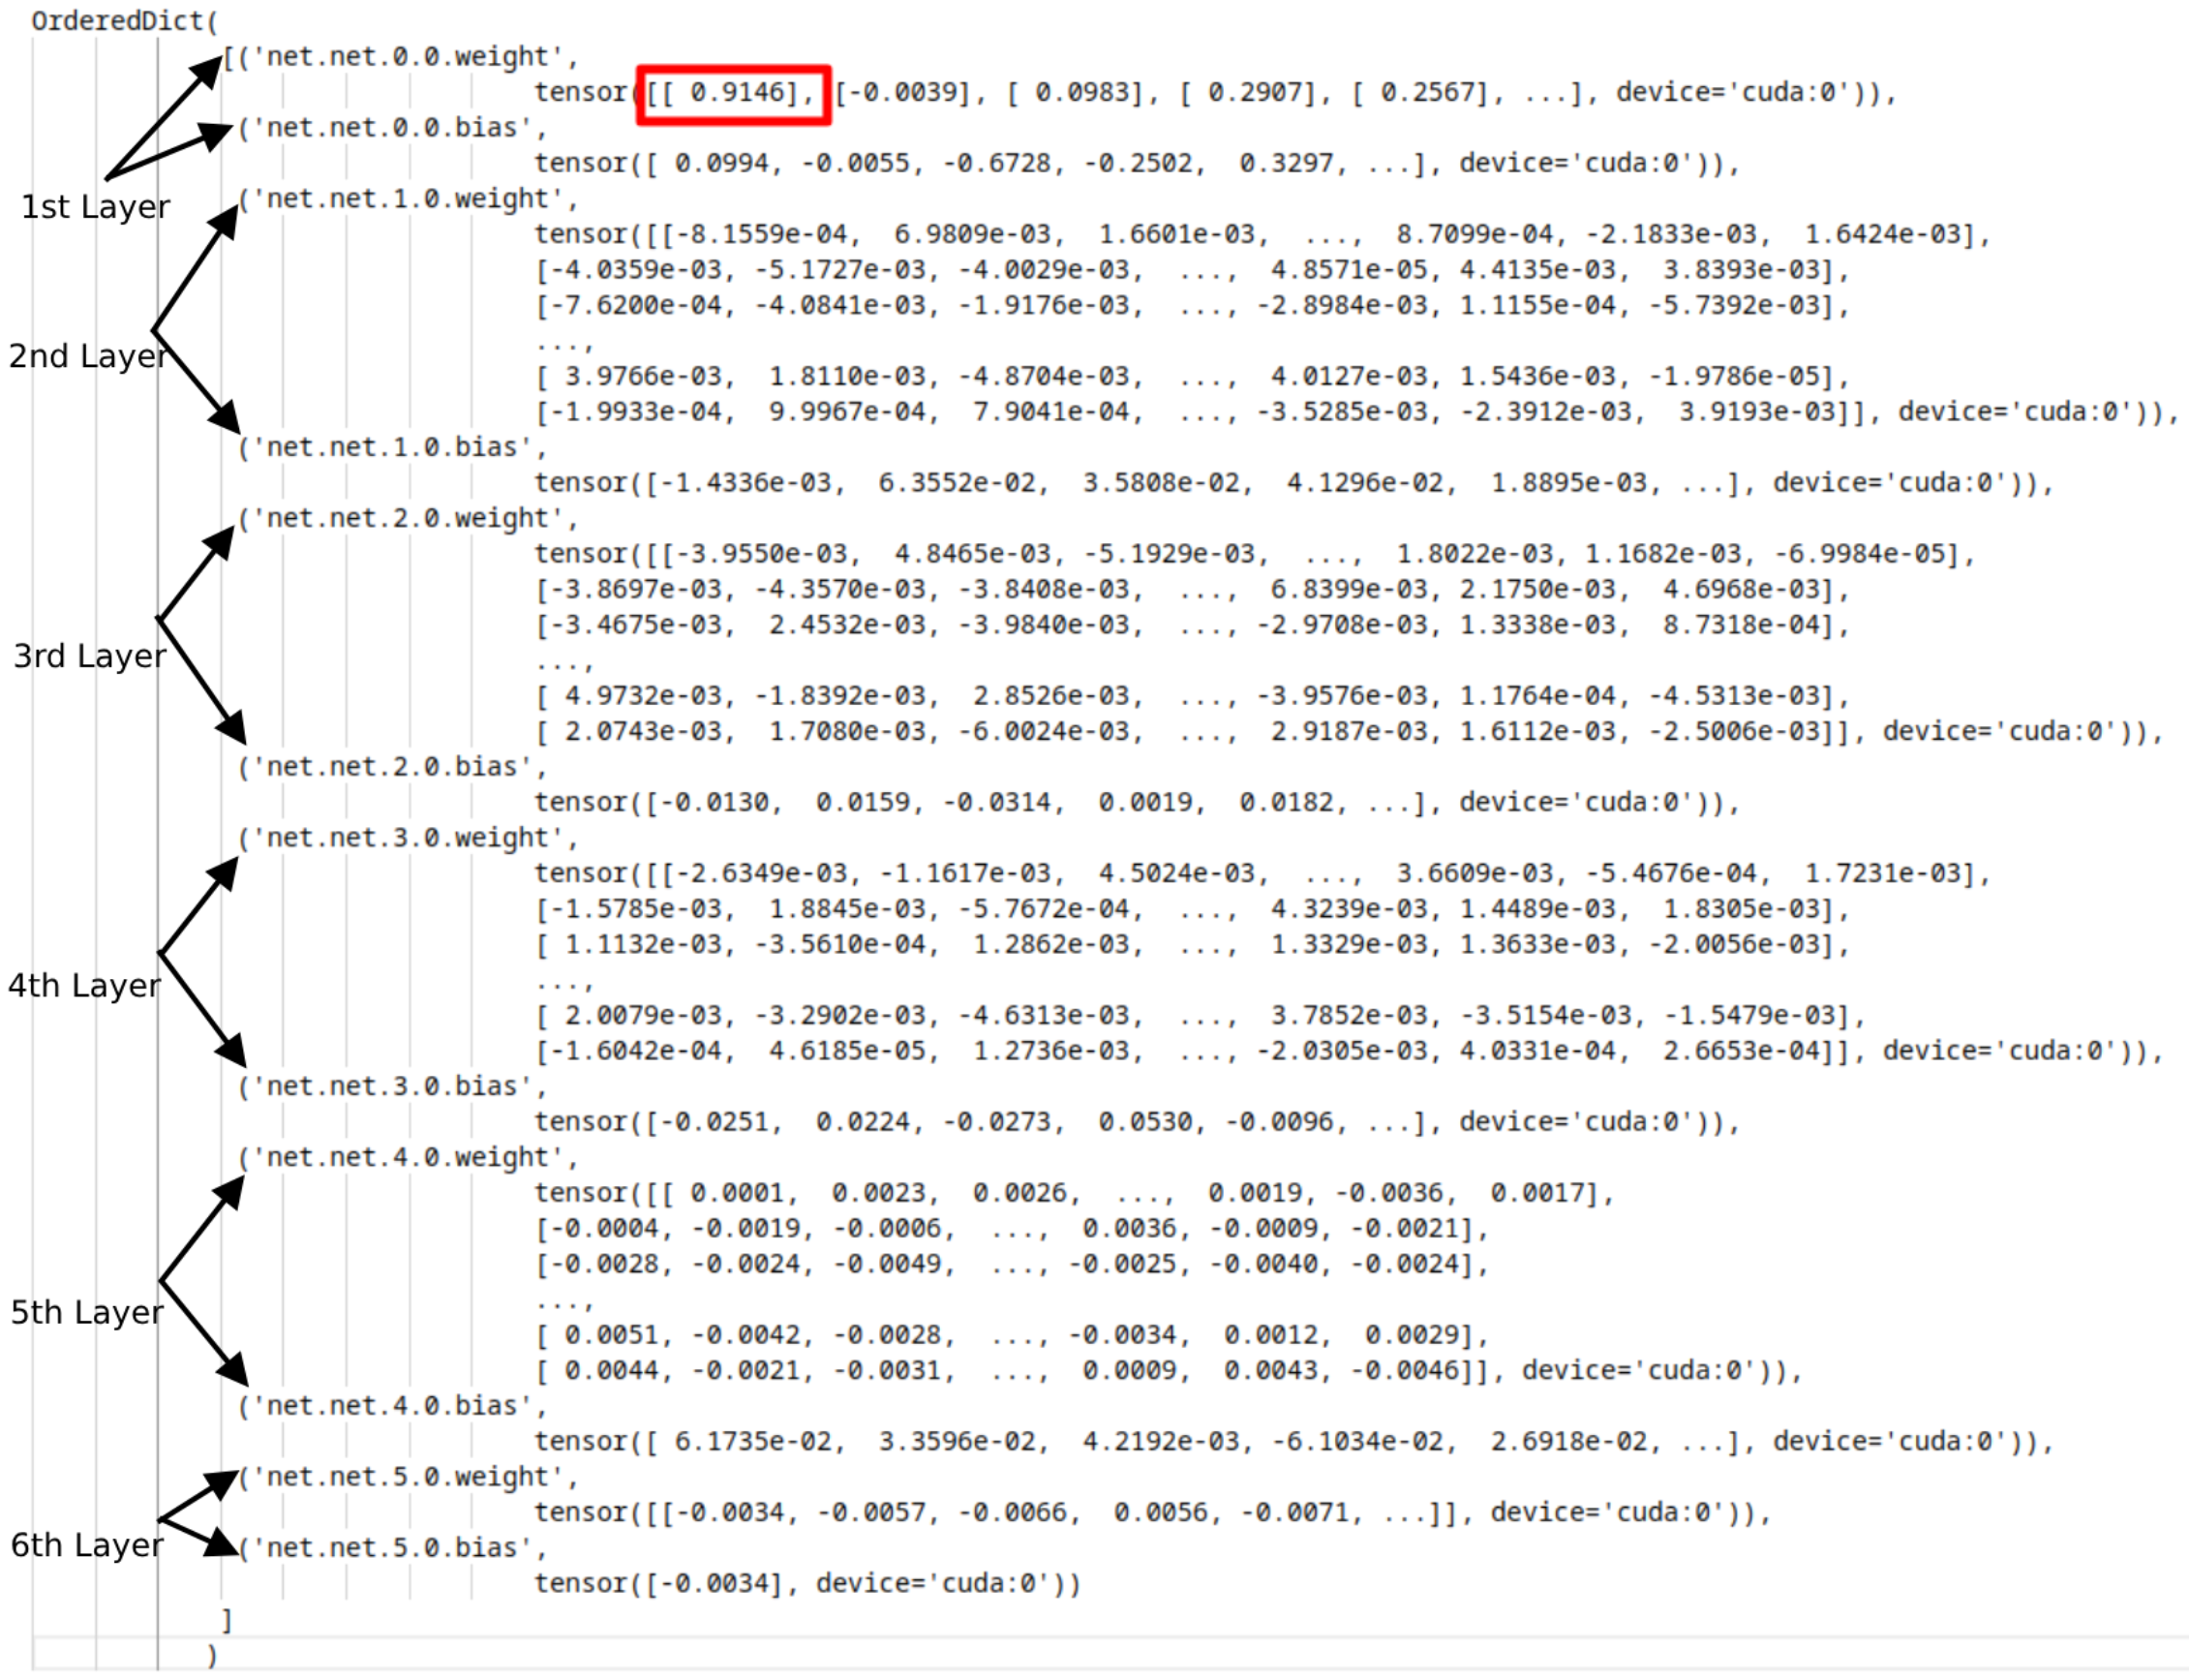
\includegraphics[width=\linewidth]{assets/weightsviz.png}
    \caption{Final Weights for Audio 1}
    \label{fig:final-weights-a1}
\end{figure}
\begin{table}[H]
    \caption{Derivation and PyTorch Notation for Weights and Biases}
    \centering
    \resizebox{\textwidth}{!}{%
    \begin{tabular}{|l|l|c|c|c|c|}
    \hline
    \multicolumn{2}{|c|}{\textbf{Layer}} & \multicolumn{2}{|c|}{\textbf{Derivation Notation}} & \multicolumn{2}{|c|}{\textbf{PyTorch Notation}} \\ \hline
    \textbf{From} & \textbf{To} & \textbf{Weights} & \textbf{Biases} & \textbf{Weights} & \textbf{Biases} \\ \hline
    Input & Input Layer & $W_{in}$ & $b_{in}$ & \texttt{net.net.0.0.weight} & \texttt{net.net.0.0.bias} \\ \hline
    Input Layer & Hidden 1 & $W^{(1)}$ & $b^{(1)}$ & \texttt{net.net.1.0.weight} & \texttt{net.net.1.0.bias} \\ \hline
    Hidden 1 & Hidden 2 & $W^{(2)}$ & $b^{(2)}$ & \texttt{net.net.2.0.weight} & \texttt{net.net.2.0.bias} \\ \hline
    Hidden 2 & Hidden 3 & $W^{(3)}$ & $b^{(3)}$ & \texttt{net.net.3.0.weight} & \texttt{net.net.3.0.bias} \\ \hline
    Hidden 3 & Hidden 4 & $W^{(4)}$ & $b^{(4)}$ & \texttt{net.net.4.0.weight} & \texttt{net.net.4.0.bias} \\ \hline
    Hidden 4 & Output & $W_{out}$ & $b_{out}$ & \texttt{net.net.5.0.weight} & \texttt{net.net.5.0.bias} \\ \hline
    \end{tabular}%
    }
    \label{table:weights_biases}
    \end{table}
    
    
To represent the number \( 0.9146 \) in IEEE 754 single precision floating-point format:

1. \textbf{Convert to Binary:}
\[
0.9146_{10} \approx 0.111010100010001100111010_2
\]

2. \textbf{Normalize the Binary Number:}
\[
0.111010100010001100111010_2 = 1.11010100010001100111010 \times 2^{-1}
\]

3. \textbf{Bias the Exponent:}
\[
\text{Exponent} = -1 + 127 = 126
\]

In binary:
\[
126_{10} = 01111110_2
\]

4. \textbf{IEEE 754 Representation:}
\begin{equation}
    \begin{array}{|c|c|c|}
        \hline
        \text{Sign Bit} & \text{Exponent} & \text{Mantissa} \\
        \hline
        0 & 01111110 & 11010100010001100111010 \\
        \hline
    \end{array}
\end{equation}

5. \textbf{Convert IEEE 754 Representation to Decimal:}
\begin{itemize}
    \item \textbf{Sign Bit}: 0 (indicating a positive number)
    \item \textbf{Exponent}: \(01111110_2\) in binary, which is 126 in decimal.
    \item \textbf{Bias}: 127
    \item \textbf{Actual Exponent}: \(126 - 127 = -1\)
    \item \textbf{Mantissa}: \(1.11010100010001100111010_2\) (implicit leading 1 added)
\end{itemize}

\textbf{Calculate the Decimal Value:}
\[
\text{Value} = (-1)^{\text{sign}} \times 1.\text{Mantissa} \times 2^{\text{Actual Exponent}}
\]
\[
\text{Value} = (-1)^0 \times 1.11010100010001100111010_2 \times 2^{-1}
\]

Convert \(1.11010100010001100111010_2\) to decimal:
\begin{align*}
    1.11010100010001100111010_2 &= 1 + 0.5 + 0.25 + 0.0625 + 0.015625 + 9.765625 \times 10^{-4}\\
        &\begin{aligned}
        % &1 + 0.5 + 0.25 + 0.0625 + 0.015625 + 9.765625 \times 10^{-4}\\
        &+ 6.103515625 \times 10^{-5} + 3.051757813 \times 10^{-5} + \\
        & 3.814697266 \times 10^{-6} + 1.907348633 \times 10^{-6}\\
        &+ 9.536743164 \times 10^{-7} + 2.384185791 \times 10^{-7}\\
    \end{aligned}\\
        &= 1.829200029373168945312
\end{align*}
\begin{equation}
    \begin{aligned}
        \text{Value} &= 1.829200029373168945312 \times 2^{-1}\\
        &= 1.829200029373168945312 \times 0.5\\
        &= 0.914600014686584472656
    \end{aligned}
\end{equation}

The discrepancy arises because the true value of \(0.9146\) cannot be exactly represented in binary. The value stored in IEEE 754 format is \(0.914600014686584472656\), which is very close to the original value \(0.9146\), with the difference due to rounding in the conversion process.

\pagebreak


\setcounter{subsection}{4}
\subsection{Custom Floating-Point Format}
\label{app:custom-floating-point-formats}
\appendixnumbering{\Alph{subsection}}

\begin{enumerate}[label=\textbf{\roman*.}]
    \item \textbf{FP32:}
    FP32 (32-bit Floating Point) is the standard floating-point format widely used in many applications, offering a good balance of precision and dynamic range. It consists of 1 sign bit, 8 exponent bits, and 23 mantissa bits, offering a high degree of precision.
    \[
    \begin{array}{|c|c|c|}
        \hline
        \text{Sign Bit} & \text{Exponent} & \text{Mantissa} \\
        \hline
        1 \text{bit} & 8 \text{bits} & 23 \text{bits} \\
        \hline
    \end{array}
    \]
    FP32 is commonly used in applications where high precision is necessary, such as scientific computing, 3D graphics, and high-performance computing.

    \textbf{Calculation of Minimum and Maximum values:}
    \[
    \text{Value} = (-1)^{\text{sign}} \times 1.\text{Mantissa} \times 2^{\text{Exponent - 127}}
    \]

    For maximum value:\\
    Sign = 0 \\
    Exponent = 11111110 (All 1s is reserved for NaN values) \\
    Mantissa = 11111111111111111111111 
    \[
        \begin{aligned}
            \text{Maximum Value} &= (-1)^{0} \times 1.11111111111111111111111 \times 2^{11111110} \\
            & \approx (1) \times 1.999999880 \times 2^{254 - 127} \\
            & \approx 1.999999880 \times 2^{127} \\
            & \approx 3.4028235 \times 10^{38}
        \end{aligned}
    \]

    For minimum value:\\
    The minimum value that can be represented in FP32 is a subnormal number. To indicate a subnormal number, all 0s are stored in Exponent. \\
    Sign = 1 \\
    Exponent = 00000000 (Indicating a subnormal number)\\
    Mantissa = 00000000000000000000001
    \[
        \begin{aligned}
            \text{Minimum Value} &= (-1)^{1} \times 0.00000000000000000000001 \times 2^{-126} \\
            & = (-1) \times 2^{-23} \times 2^{-126} \\
            & =  2^{-149} \\
            & \approx -1.401298 \times 10^{-45}
        \end{aligned}
    \]
    The minimum normal value can also be calculated as : \\
    Sign = 1 \\
    Exponent = 00000001 (Smallest non-zero exponent for normalized numbers)\\
    Mantissa = 00000000000000000000000
    \[
        \begin{aligned}
            \text{Minimum Value} &= (-1)^{1} \times 1 \times 2^{-126} \\
            & = (-1) \times (1) \times 2^{-126} \\
            & =  -2^{-126} \\
            & \approx -1.1754944 \times 10^{-38}
        \end{aligned}
    \]

    \begin{table}[H]
        \centering
        \caption{Advantages and Disadvantages of FP32}
        \label{tab:fp32}
        \begin{tabular}{|p{6cm}|p{6cm}|}
        \hline
        \textbf{Advantages} & \textbf{Disadvantages} \\
        \hline
        High Precision: Suitable for applications requiring high numerical accuracy. & Computationally Expensive: Requires more memory and processing power. \\
        \hline
        Wide Dynamic Range: Supports a wide range of values. & Slower Operations: More resource-intensive than lower precision formats. \\
        \hline
        \end{tabular}
    \end{table}

\item \textbf{FP16:}
    FP16 (16-bit Floating Point) is a lower-precision floating-point format that sacrifices some precision in favor of reducing memory usage and improving computation speed. It uses 1 sign bit, 5 exponent bits, and 10 mantissa bits.
    \[
    \begin{array}{|c|c|c|}
        \hline
        \text{Sign Bit} & \text{Exponent} & \text{Mantissa} \\
        \hline
        1 \text{bit} & 5 \text{bits} & 10 \text{bits} \\
        \hline
    \end{array}
    \]
    
    FP16 is commonly used in machine learning tasks to speed up training while reducing memory consumption.

    \textbf{Calculation of Minimum and Maximum values:}
    \[
    \text{Value} = (-1)^{\text{sign}} \times 1.\text{Mantissa} \times 2^{\text{Exponent - 15}}
    \]

    For maximum value:\\
    Sign = 0 \\
    Exponent = 11110 (All 1s is reserved for NaN values) \\
    Mantissa = 1111111111 
    \[
        \begin{aligned}
            \text{Maximum Value} &= (-1)^{0} \times 1.1111111111 \times 2^{11110} \\
            & \approx (1) \times 1.999999880 \times 2^{30 - 15} \\
            & \approx 1.999999880 \times 2^{15} \\
            & \approx 65504
        \end{aligned}
    \]

    For minimum value:\\
    The minimum value that can be represented in FP16 is a subnormal number. To indicate a subnormal number, all 0s are stored in Exponent. \\
    Sign = 1 \\
    Exponent = 00000 (Indicating a subnormal number)\\
    Mantissa = 0000000001
    \[
        \begin{aligned}
            \text{Minimum Value} &= (-1)^{1} \times 0.0000000001 \times 2^{-14} \\
            & = (-1) \times 2^{-10} \times 2^{-14} \\
            & =  2^{-24} \\
            & \approx -5.960464477 \times 10^{-8}
        \end{aligned}
    \]
    The minimum normal value can also be calculated as : \\
    Sign = 1 \\
    Exponent = 00001 (Smallest non-zero exponent for normalized numbers)\\
    Mantissa = 0000000000
    \[
        \begin{aligned}
            \text{Minimum Value} &= (-1)^{1} \times 1 \times 2^{-14} \\
            & = (-1) \times (1) \times 2^{-15} \\
            & =  -2^{-15} \\
            & \approx -3.051757 \times 10^{-5}
        \end{aligned}
    \]

 
    \begin{table}[H]
        \centering
        \caption{Advantages and Disadvantages of FP16}
        \label{tab:fp16}
        \begin{tabular}{|p{6cm}|p{6cm}|}
        \hline
        \textbf{Advantages} & \textbf{Disadvantages} \\
        \hline
        Reduced Memory Usage: Saves memory space, especially for large models. & Lower Precision: Less accurate for some tasks requiring high precision. \\
        \hline
        Faster Computation: Reduces processing time in many tasks. & Limited Dynamic Range: Smaller exponent range than FP32. \\
        \hline
        \end{tabular}
    \end{table}

\item \textbf{FP8:}
    FP8 (8-bit Floating Point) is an extremely low-precision format that is mainly used in specialized applications where extreme memory efficiency is required. It uses 1 sign bit, 4 exponent bits, and 3 mantissa bits.
    \[
    \begin{array}{|c|c|c|}
        \hline
        \text{Sign Bit} & \text{Exponent} & \text{Mantissa} \\
        \hline
        1 \text{bit} & 4 \text{bits} & 3 \text{bits} \\
        \hline
    \end{array}
    \]
    The above example is of E4M3 variant. It also has another variant named E5M2 which has 1 sign bit, 5 exponent bits and only 2 mantissa bits.
    
    FP8 is used in contexts like model quantization or inference tasks, where the trade-off between precision and speed can be adjusted.

    \textbf{Calculation of Minimum and Maximum values(E4M3):}
    
    \[
    \text{Value} = (-1)^{\text{sign}} \times 1.\text{Mantissa} \times 2^{\text{Exponent - 7}}
    \]

    For maximum value:\\
    Sign = 0 \\
    Exponent = 1111 \\
    Mantissa = 110
    \[
    \begin{aligned}
        \text{Maximum Value} &= (-1)^{0} \times 1.110 \times 2^{1110} \\
        &= (1) \times 1.75 \times 2^{15 - 7} \\
        &= 1.75 \times 2^{8} \\
        &= 1.75 \times 128 \\
        &= 448
    \end{aligned}
    \]
    
    For minimum value:\\
    The minimum value that can be represented in FP8 is a subnormal number. To indicate a subnormal number, all 0s are stored in Exponent. \\
    Sign = 1 \\
    Exponent = 0000 (All 1s is reserved for NaN values) \\
    Mantissa = 111 
    \[
    \begin{aligned}
        \text{Minimum Value} &= (-1)^{1} \times 0.111 \times 2^{-6} \\
        &= (-1) \times 0.875 \times 2^{-6} \\
        &= -1.875 \times 2^{-6} \\
        &= -1.875 \times 128 \\
        & \approx -1.36 \times 10^{-2}
    \end{aligned}
    \]
    The minimum normal value can also be calculated as : \\
    Sign = 1 \\
    Exponent = 0001 (Smallest non-zero exponent for normalized numbers)\\
    Mantissa = 000
    \[
        \begin{aligned}
            \text{Minimum Value} &= (-1)^{1} \times 1 \times 2^{-6} \\
            & =  -2^{-6} \\
            & \approx -1.56 \times 10^{-2}
        \end{aligned}
    \]

 
    \begin{table}[H]
        \centering
        \caption{Advantages and Disadvantages of FP8}
        \label{tab:fp8}
        \begin{tabular}{|p{6cm}|p{6cm}|}
        \hline
        \textbf{Advantages} & \textbf{Disadvantages} \\
        \hline
        Extremely Low Memory Usage: Minimizes memory requirements. & Very Low Precision: Inadequate for tasks requiring high accuracy. \\
        \hline
        Faster Computation: Significantly increases speed in simple operations. & Small Dynamic Range: Can lead to overflows and underflows. \\
        \hline
        Reduced data movement and simpler arithmetic operations lead to lower power consumption. & Limited Support : FP8 is not yet supported by all hardware and software \\
        \hline
        \end{tabular}
    \end{table}

    \item \textbf{INT8:}
    INT8 (8-bit Integer) is a format that uses 8 bits to represent integers in the range from -128 to 127. It is primarily used in tasks requiring integer values, like certain parts of machine learning models, especially in quantization.
    \[
    \begin{array}{|c|c|}
        \hline
        \text{Sign Bit} & \text{Magnitude} \\
        \hline
        1 \text{bit} & 7 \text{bits} \\
        \hline
    \end{array}
    \]
    
    int8 is widely used for model quantization, where it is employed to significantly reduce the memory footprint and increase computational efficiency.

    \textbf{Calculation of Minimum and Maximum values:} 
    \begin{enumerate}
        \item For Signed INT8:
        \begin{itemize}
            \item Maximum Value:\\
            Sign = 0 \\
            Magnitude = 1111111
                \[
                \begin{aligned}
                    \text{Maximum Value} &= (-1)^{0} \times 1111111 \\
                    &= 127
                \end{aligned}
                \]
            \item Minimum Value:\\
            Sign = 1 \\
            Magnitude = 0000000 
                \[
                \begin{aligned}
                    \text{Minimum Value} &= (-1)^{1} \times 128 (\text{2s complement of} 10000000)\\
                    &= -128
                \end{aligned}
                \]
            \end{itemize}
    \item For Unsigned INT8: 
            \begin{itemize}
                \item Maximum Value:\\
            Sign = 0 \\
            Magnitude = 11111111
                \[
                \begin{aligned}
                    \text{Maximum Value} &= 11111111 \\
                    &=255
                \end{aligned}
                \]
            \item Minimum Value:\\
            Sign = 0 \\
            Magnitude = 00000000 
                \[
                \begin{aligned}
                    \text{Minimum Value} &= 0
                \end{aligned}
            \]
            \end{itemize}
    \end{enumerate}

 
    \begin{table}[H]
        \centering
        \caption{Advantages and Disadvantages of int8}
        \label{tab:int8}
        \begin{tabular}{|p{6cm}|p{6cm}|}
        \hline
        \textbf{Advantages} & \textbf{Disadvantages} \\
        \hline
        Extremely Low Memory Usage: Uses minimal memory, ideal for embedded systems. & Very Low Range: Limited to integer values, with no fractional precision. \\
        \hline
        High-Speed Computation: Operates very quickly in suitable tasks. & Precision Loss: Can cause inaccuracies in tasks that require floating-point precision. \\
        \hline
        \end{tabular}
    \end{table}

    \item \textbf{bfloat16:}
    BFLOAT16 (Brain Floating Point Format) is a custom 16-bit floating-point format primarily developed by Google. It uses the same 8-bit exponent as FP32 but reduces the mantissa to 7 bits, compared to 23 bits in FP32.
    \[
    \begin{array}{|c|c|c|}
        \hline
        \text{Sign Bit} & \text{Exponent} & \text{Mantissa} \\
        \hline
        1 \text{bit} & 8 \text{bits} & 7 \text{bits} \\
        \hline
    \end{array}
    \]
    
    BFLOAT16 was introduced to address computational and memory bottlenecks in deep learning and high-performance computing. Many machine learning tasks do not require the precision of FP32, leading to unnecessary computational overhead. By reducing the mantissa size, bfloat16 allows for faster computation and reduced memory usage while maintaining the dynamic range of FP32. \\
    \textbf{Calculation of Minimum and Maximum values:} 
    \[
    \text{Value} = (-1)^{\text{sign}} \times 1.\text{Mantissa} \times 2^{\text{Exponent - 127}}
    \]

    For maximum value:\\
    Sign = 0 \\
    Exponent = 11111110 \ (\text{All 1s is reserved for NaN values}) \\
    Mantissa = 1111111
    \[
        \begin{aligned}
            \text{Maximum Value} &= (-1)^{0} \times 1.1111111 \times 2^{11111110} \\
            & \approx (1) \times 1.9921875 \times 2^{254 - 127} \\
            & \approx 1.9921875 \times 2^{127} \\
            & \approx 3.3895314 \times 10^{38}
        \end{aligned}
    \]

    For minimum value:\\
    The minimum value in BFLOAT16 is a subnormal number. To indicate a subnormal number, all 0s are stored in Exponent. \\
    Sign = 1 \\
    Exponent = 00000000 \ (\text{Indicating a subnormal number}) \\
    Mantissa = 0000001
    \[
        \begin{aligned}
            \text{Minimum Value} &= (-1)^{1} \times 0.0000001 \times 2^{-126} \\
            & = (-1) \times 2^{-7} \times 2^{-126} \\
            & = -2^{-133} \\
            & \approx -9.1835496 \times 10^{-41}
        \end{aligned}
    \]
    The minimum normal value can also be calculated as:

        Sign = 1 \\
        Exponent = 00000001 (Smallest non-zero exponent for normalized numbers) \\
        Mantissa = 0000000

    \[
        \begin{aligned}
            \text{Minimum Value} &= (-1)^{1} \times 1.0000000 \times 2^{-126} \\
            & = (-1) \times (1) \times 2^{-126} \\
            & =  -2^{-126} \\
            & \approx -1.175494 \times 10^{-38}
        \end{aligned}
    \]

    \begin{table}[H]
        \centering
        \caption{Advantages and Disadvantages of BFLOAT16}
        \label{tab:bfloat16}
            \begin{tabular}{|p{6cm}|p{6cm}|}
            \hline
            \textbf{Advantages} & \textbf{Disadvantages} \\
            \hline
            Wide Dynamic Range: Retains the same exponent range as fp32, reducing overflow and underflow. & Reduced Precision: Smaller mantissa affects operations requiring high accuracy. \\
            \hline
            Computational Efficiency: Reduces memory usage and increases computation speed. & 
            Software/Hardware Dependency: Requires specialized support.\\
            \hline
            \end{tabular}
    \end{table}

    \item \textbf{TF32:}
    TF32 (TensorFloat-32) is a custom precision format introduced by NVIDIA. It uses the same 8-bit exponent as FP32 but reduces the mantissa to 10 bits.
    \[
    \begin{array}{|c|c|c|}
        \hline
        \text{Sign Bit} & \text{Exponent} & \text{Mantissa} \\
        \hline
        1 \text{bit} & 8 \text{bits} & 10 \text{bits} \\
        \hline
    \end{array}
    \]

    TF32 is specifically designed to accelerate tensor computations in machine learning while maintaining sufficient precision for stable training. TF32 bridges the gap between performance and precision in deep learning. While FP32 operations are computationally expensive and FP16 lacks the precision needed for complex model training, TF32 offers a middle ground by maintaining the exponent range of FP32 and reducing the mantissa size to speed up tensor operations.
    \textbf{Calculation of Minimum and Maximum values:} 
    \[
        \text{Value} = (-1)^{\text{sign}} \times 1.\text{Mantissa} \times 2^{\text{Exponent - 127}}
    \]

    For maximum value:\\
    Sign = 0 \\
    Exponent = 11111110 \ (\text{Maximum exponent for normalized numbers}) \\
    Mantissa = 1111111111
    \[
        \begin{aligned}
            \text{Maximum Value} &= (-1)^{0} \times 1.1111111111 \times 2^{11111110} \\
            & \approx (1) \times 1.9990234 \times 2^{254 - 127} \\
            & \approx 1.9990234 \times 2^{127} \\
            & \approx 3.4011621 \times 10^{38}
        \end{aligned}
    \]

    For minimum value:\\

    Sign = 1 \\
    Exponent = 00000001 \\
    Mantissa = 1111111111
    \[
        \begin{aligned}
            \text{Minimum Value} &= (-1)^{1} \times 1.1111111111 \times 2^{-126} \\
            & = (-1) \times (1) \times 2^{-126} \\
            & =  -2^{-126} \\
            & \approx -1.175494 \times 10^{-38}
        \end{aligned}
    \]

    \begin{table}[H]
        \centering
        \caption{Advantages and Disadvantages of TF32}
        \label{tab:tf32}
        \begin{tabular}{|p{6cm}|p{6cm}|}
        \hline
        \textbf{Advantages} & \textbf{Disadvantages} \\
        \hline
        Performance Gains: Faster tensor operations and matrix multiplications. & Less Precision than FP32: Unsuitable for applications needing high numerical accuracy. \\
        \hline
        Precision-Performance Balance: Sufficient precision for most training tasks. & Limited to NVIDIA GPUs: Proprietary format tied to specific hardware. \\
        \hline
        \end{tabular}
        \end{table}
        
\end{enumerate}

\pagebreak


\setcounter{subsection}{5}
\subsection{Quantization with Example}
\label{app:quantization-manual-conversion}
\appendixnumbering{\Alph{subsection}}

Quantization is a technique used in machine learning to reduce the precision of numbers used in computations and storage. There are two primary types of quantization: symmetric and asymmetric. Below is a detailed explanation of asymmetric quantization.

\subsubsection{Asymmetric Quantization}
\begin{figure}[H]
    \centering
    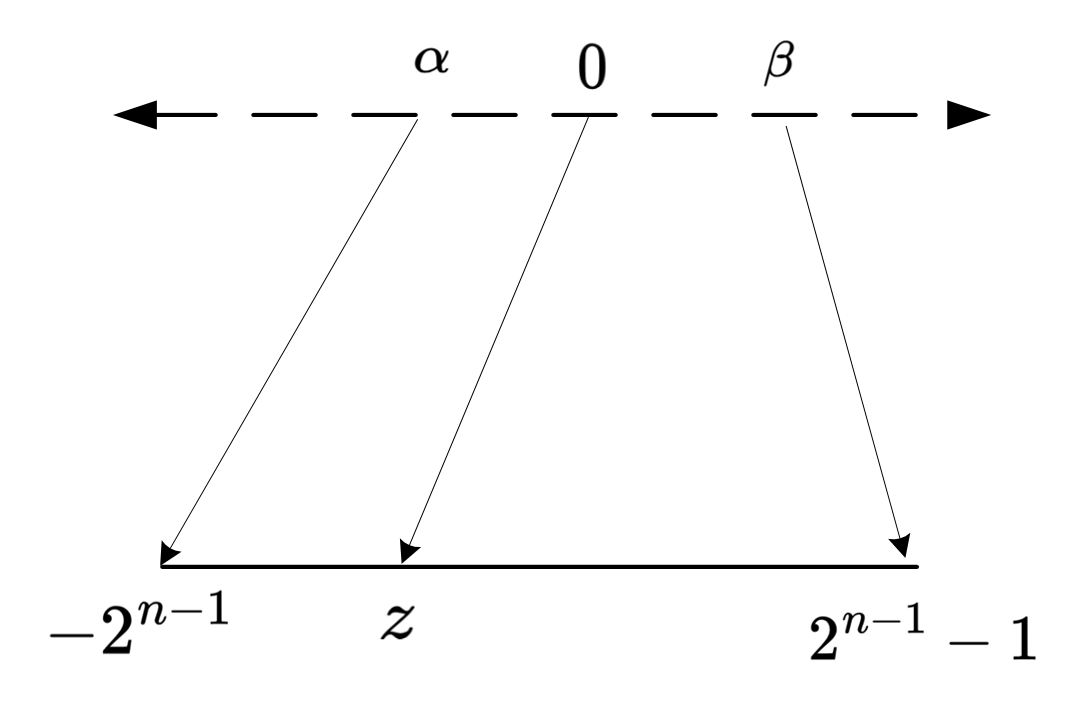
\includegraphics[width=0.7\linewidth]{assets/quantization/Unsymmetric_Qfigure.png}
    \caption{Asymmetric Quantization}
    \label{fig:Unsymmetric_Qfigure}
\end{figure}
In asymmetric quantization, the range of values is not necessarily symmetric around zero. This allows the representation of values that are skewed toward either positive or negative numbers.

\textbf{Characteristics:}
\begin{enumerate}
    \item The zero point is not fixed at zero; it is a non-zero number that provides offset of zero.
    \item Both scale and zero point are required to calculate quantized value.
    \[
        \text{quantized value} = \text{round}\left(\frac{\text{original value}}{\text{scale}} + \text{zero-point}\right)
    \]
    where,
        \[
            \text{scale} = \frac{w_{\text{max}} - w_{\text{min}}}{2^n - 1}
        \]
        \[
            \text{zero-point} = q_{\text{min}} - \frac{w_{\text{min}}}{\text{scale}}
        \]
\end{enumerate}

Then the dequantized value can be calculated as:
\[ \text{dequantized value} = (\text{quantized value} - \text{zero-point}) \cdot \text{scale} \]

\begin{table}[H]
    \centering
    \caption{Comparison of Symmetric and Asymmetric Quantization}
    \label{tab:quantization_comparison}
    \begin{tabularx}{\textwidth}{|l|X|X|}
    \hline
    \textbf{Aspect} & \textbf{Symmetric Quantization} & \textbf{Asymmetric Quantization} \\ \hline
    \textbf{Use Cases} &
    - Neural network weights (often symmetrically distributed). \newline
    - Scenarios requiring simple computations. \newline
    - Signed data distributions centered around zero. &
    - Input activations in neural networks. \newline
    - Data with skewed or biased distributions (e.g., image pixel values).\\ \hline
    
    \textbf{Advantages} &
    - Simpler arithmetic due to zero-point being zero. \newline
    - Efficient for hardware implementations using signed integers (e.g., int8). \newline
    - Ideal for symmetric data distributions. &
    - Better range utilization for skewed data. \newline
    - Reduces quantization error for asymmetric distributions. \newline
    - Improved accuracy for biased data. \\ \hline
    
    \textbf{Disadvantages} &
    - Inefficient for asymmetric data distributions. \newline
    - May lead to higher quantization error for skewed data. &
    - More complex arithmetic due to non-zero zero-point. \newline
    - Slightly higher computational overhead. \newline
    - Hardware may require additional complexity to implement. \\ \hline
    \end{tabularx}
\end{table}

\subsubsection{Quantization to 8-bit Integer Format}
We will demonstrate an example of asymmetric quantization, and symmetric quantization can then be easily derived from this example.
Given the following values:
\begin{align}
\text{original value} &= 0.14893225 \\
\text{scale} &= 0.002625829565758799 \\
\text{zero-point} &= -0.23390677845551977
\end{align}

\textbf{Substitute the values into the formula:}
\[
\text{quantized value} = \text{round}\left(\frac{0.14893225}{0.002625829565758799} - 0.23390677845551977\right)
\]

\textbf{Calculate step-by-step:}
\[
\frac{0.14893225}{0.002625829565758799} \approx 56.7181708753
\]
Now, adding zero-point,
\[ 56.69868081 + -0.23390677845551977 \approx 56.4842640968 \]

Thus we get,
\begin{equation}
    \begin{aligned}
        \text{quantized value} &= \text{round}(56.46477403) \\
        &= \boxed{56}
    \end{aligned}
\end{equation}

\subsubsection{Dequantization to 32-bit Floating-Point Format}

Given the formula for dequantization:
\[
\text{dequantized value} = (\text{quantized value} - \text{zero-point}) \times \text{scale}
\]

\textbf{Substitute the values:}
\[
\text{dequantized value} = (56 - (-0.23390677845551977)) \times 0.002625829565758799
\]

\textbf{Calculate step-by-step:}
\[
56 - (-0.23390677845551977) = 56 + 0.23390677845551977
                         \approx 56.23390678
\]

Thus we get,
\begin{equation}
    \begin{aligned}
    \text{dequantized value} &= 56.23390678 \times 0.002625829565758799\\
                            &\approx 0.14766065501\\
    \text{dequantized value} &\approx \boxed{0.14766}
    \end{aligned}
\end{equation}

\subsubsection{Quantization Error}

The quantization error is given by:
\[
\text{quantization error} = \text{original value} - \text{dequantized value}
\]

Substituting the values:
\begin{equation} 
    \begin{aligned}
        \text{quantization error} &= 0.14893225 - 0.14766065501\\
        &= 0.00127159499\\
        \text{quantization error} &\approx \boxed{0.00127}
    \end{aligned}
\end{equation}

\subsubsection{Mean Squared Quantization Error (MSQE)}
For the given data, we can now calulate \gls{msqe} and see how quantization error increases as integer bit-width decreases as shown in \autoref{tab:quantization_error_reduction}.
\[
\text{Original Tensor:} \quad \mathbf{T} = \begin{bmatrix}
-0.41067, \dots, -0.92187
\end{bmatrix}
\]

\begin{table}[H]
    \centering
    \caption{Increase in Quantization Error with Lower Bit-width Integers}
    \label{tab:quantization_error_reduction}
    \begin{tabular}{|c|c|c|c|c|}
    \hline
    \textbf{Bit-width} & \textbf{Scale} & \textbf{Zero Point} & \textbf{Quantized Tensor} & \textbf{\gls{msqe}} \\ \hline
    32 & $3.48 \times 10^{-10}$ & $4.99 \times 10^8$ & $[-679681118, \dots, -2147483648]$ & $6.82 \times 10^{-21}$ \\ \hline
    16 & $2.28 \times 10^{-5}$  & $7620.56$           & $[-10371, \dots, -32768]$          & $3.86 \times 10^{-11}$ \\ \hline
    8  & $5.87 \times 10^{-3}$  & $29.15$             & $[-41, \dots, -128]$               & $1.67 \times 10^{-6}$  \\ \hline
    \end{tabular}
\end{table}

As the bit-width decreases, the quantization error increases due to the reduced precision in representing the original floating-point values. With fewer bits available to represent the data, the quantization process introduces more significant rounding errors, leading to a higher \gls{msqe}. This trade-off between precision and memory efficiency is a common consideration in quantization techniques, where the goal is to minimize the error while reducing the memory footprint of the data.

\begin{figure}[H]
    \centering
    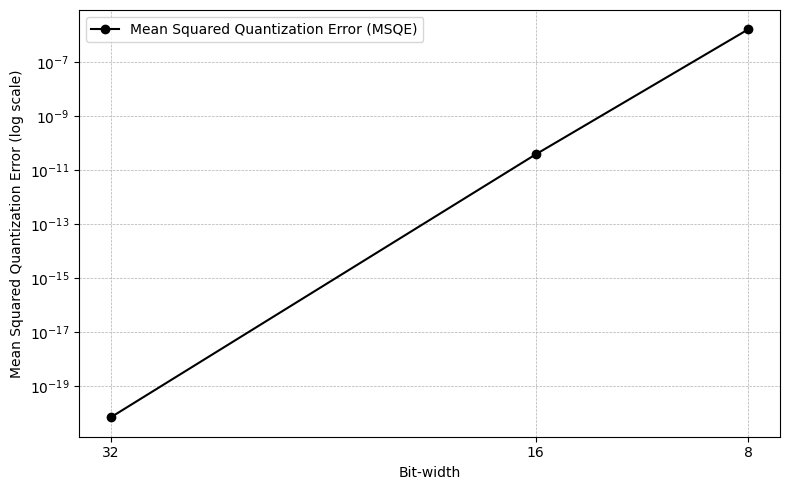
\includegraphics[width=\linewidth]{assets/quantization/MSQE_Quantization.png}
    \caption{MSQE vs Bit-width for Quantization}
    \label{fig:msqe-vs-bitwidth}
\end{figure}

\pagebreak


% References (IEEE style)
\bibliographystyle{IEEEtran}  % Use IEEE bibliography style
\bibliography{refs}     % Specify your .bib file
\addcontentsline{toc}{section}{References}
